\documentclass{standalone}
\usepackage{tikz}
\usetikzlibrary{patterns, positioning}
\usepackage[sfdefault]{ClearSans} %% option 'sfdefault' activates Clear Sans as the default text font
\usepackage[T1]{fontenc}

\begin{document}
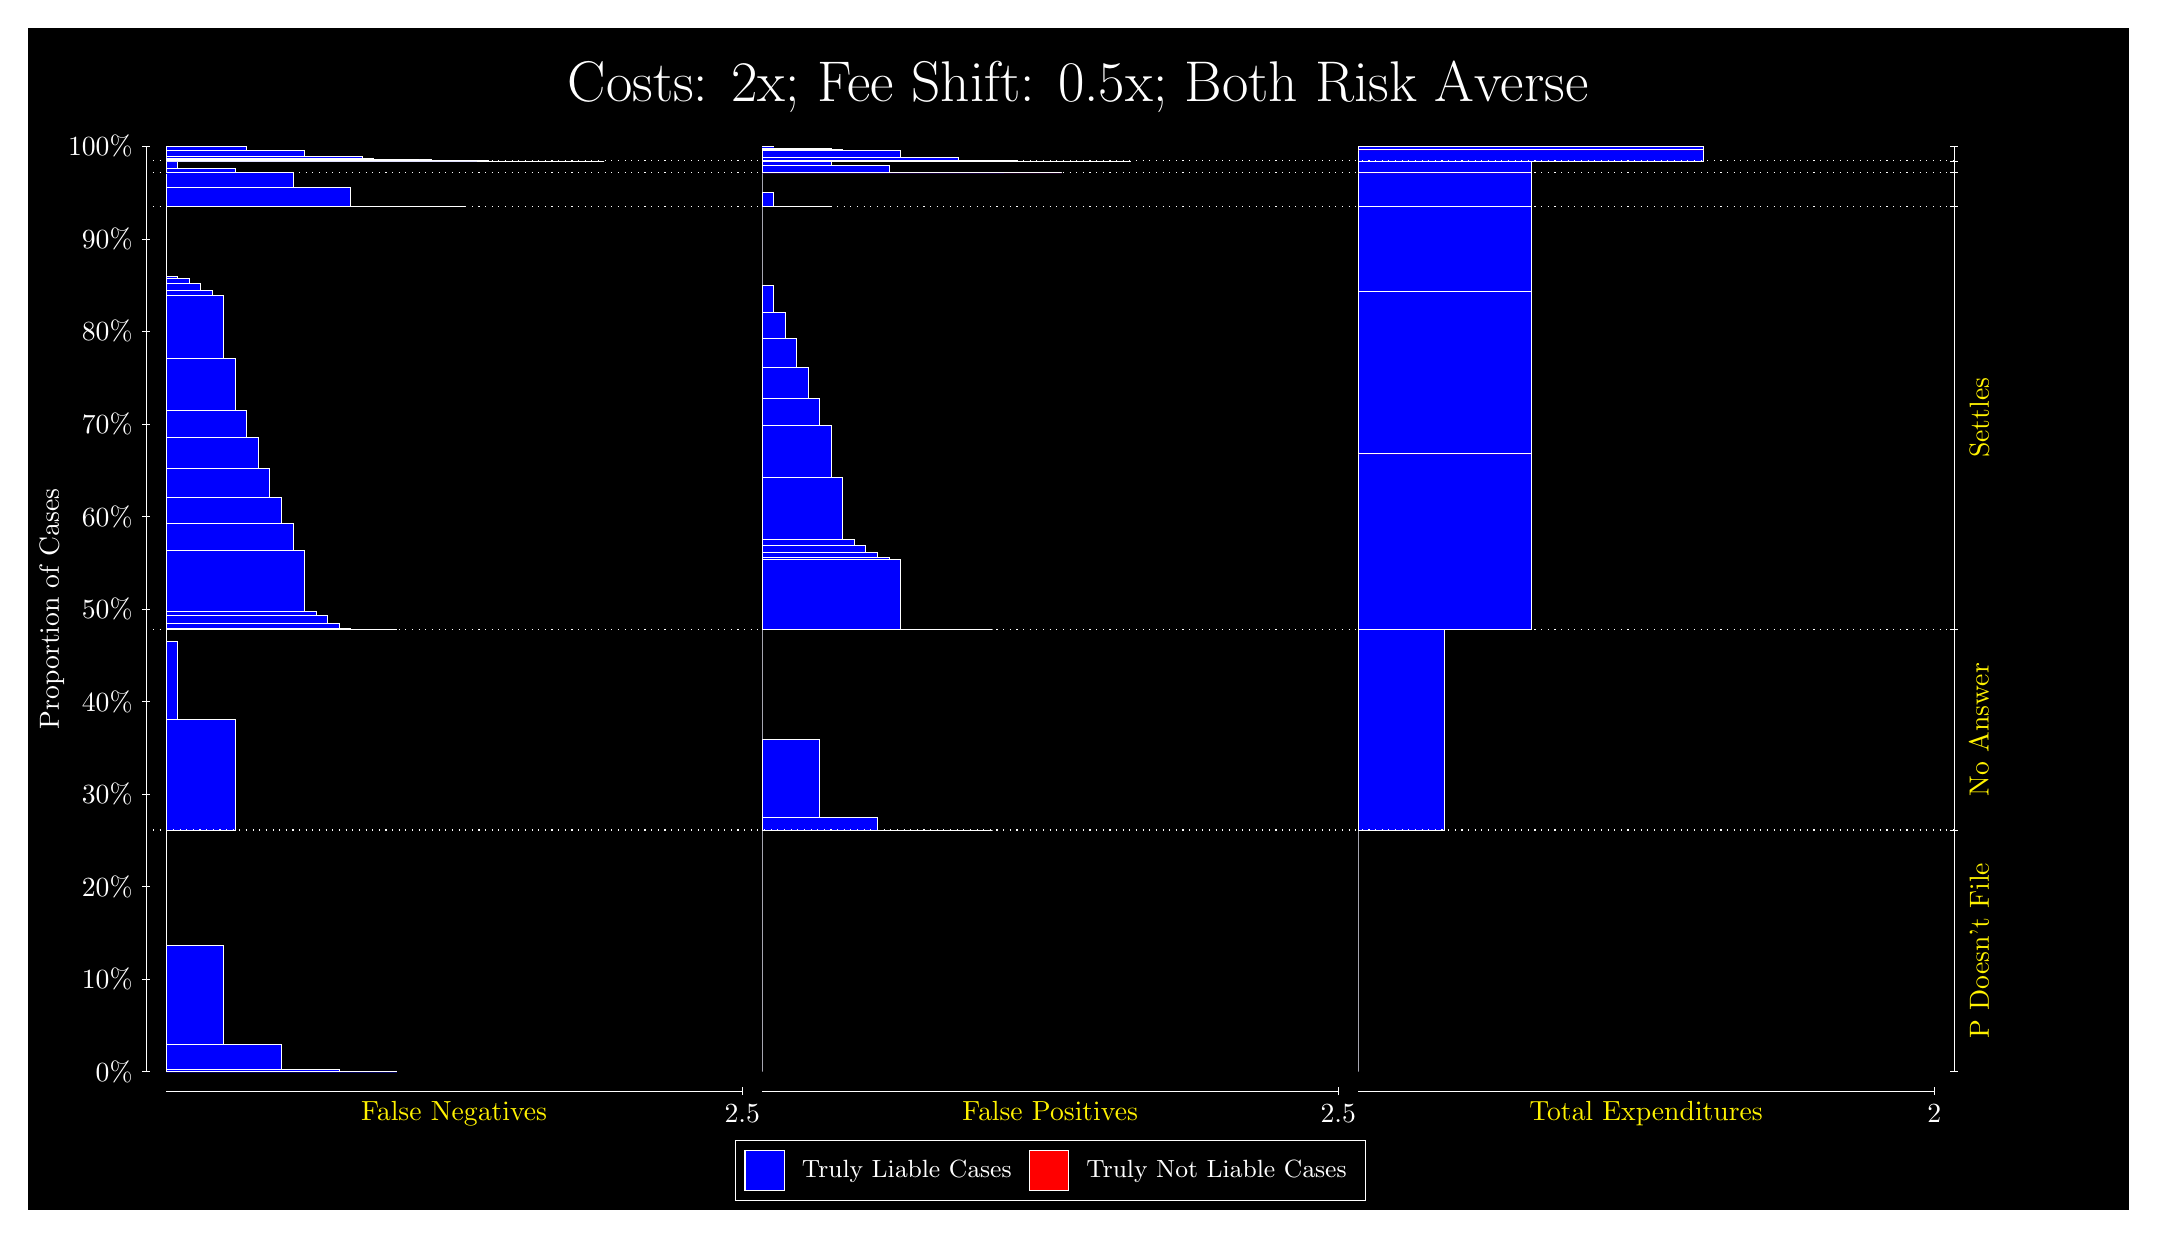
\begin{tikzpicture}
\draw[fill=black] (0,0) rectangle (26.667,15);
\draw[text=white] (0,13.5) rectangle (26.667,15) node[midway] {\huge Costs: 2x; Fee Shift: 0.5x; Both Risk Averse};
\draw[white, very thin] (1.5,1.75) -- (1.5,13.5);
\node[rotate=90, text=white, anchor=center] at (0.3, 7.625) {Proportion of Cases};
\draw[white, very thin] (1.45,1.75) -- (1.55,1.75);
\node[text=white, anchor=east] at (1.45, 1.75) {0\%};
\draw[white, very thin] (1.45,2.925) -- (1.55,2.925);
\node[text=white, anchor=east] at (1.45, 2.925) {10\%};
\draw[white, very thin] (1.45,4.1) -- (1.55,4.1);
\node[text=white, anchor=east] at (1.45, 4.1) {20\%};
\draw[white, very thin] (1.45,5.275) -- (1.55,5.275);
\node[text=white, anchor=east] at (1.45, 5.275) {30\%};
\draw[white, very thin] (1.45,6.45) -- (1.55,6.45);
\node[text=white, anchor=east] at (1.45, 6.45) {40\%};
\draw[white, very thin] (1.45,7.625) -- (1.55,7.625);
\node[text=white, anchor=east] at (1.45, 7.625) {50\%};
\draw[white, very thin] (1.45,8.8) -- (1.55,8.8);
\node[text=white, anchor=east] at (1.45, 8.8) {60\%};
\draw[white, very thin] (1.45,9.975) -- (1.55,9.975);
\node[text=white, anchor=east] at (1.45, 9.975) {70\%};
\draw[white, very thin] (1.45,11.15) -- (1.55,11.15);
\node[text=white, anchor=east] at (1.45, 11.15) {80\%};
\draw[white, very thin] (1.45,12.325) -- (1.55,12.325);
\node[text=white, anchor=east] at (1.45, 12.325) {90\%};
\draw[white, very thin] (1.45,13.5) -- (1.55,13.5);
\node[text=white, anchor=east] at (1.45, 13.5) {100\%};

\draw[white, very thin] (24.457,1.75) -- (24.457,13.5);
\draw[white, very thin] (24.407,1.75) -- (24.507,1.75);
\node[anchor=west] at (24.407, 1.75) {};
\draw[white, very thin] (24.407,4.8178) -- (24.507,4.8178);
\node[anchor=west] at (24.407, 4.8178) {};
\draw[white, very thin] (24.407,7.3693) -- (24.507,7.3693);
\node[anchor=west] at (24.407, 7.3693) {};
\draw[white, very thin] (24.407,12.738) -- (24.507,12.738);
\node[anchor=west] at (24.407, 12.738) {};
\draw[white, very thin] (24.407,13.167) -- (24.507,13.167);
\node[anchor=west] at (24.407, 13.167) {};
\draw[white, very thin] (24.407,13.315) -- (24.507,13.315);
\node[anchor=west] at (24.407, 13.315) {};
\draw[white, very thin] (24.407,13.5) -- (24.507,13.5);
\node[anchor=west] at (24.407, 13.5) {};

\draw[white, very thin, fill=blue] (1.75,1.75) rectangle (4.6775,1.7502);
\draw[white, very thin, fill=blue] (1.75,1.7502) rectangle (3.9457,1.7728);
\draw[white, very thin, fill=blue] (1.75,1.7728) rectangle (3.2138,2.0951);
\draw[white, very thin, fill=blue] (1.75,2.0951) rectangle (2.4819,3.3512);
\draw[white, very thin, fill=red] (1.75,3.3512) rectangle (1.75,3.3512);
\draw[white, very thin, fill=blue] (1.75,3.3512) rectangle (1.75,4.8178);
\draw[white, very thin, fill=blue] (1.75,4.8178) rectangle (2.6283,6.2185);
\draw[white, very thin, fill=blue] (1.75,6.2185) rectangle (1.8964,7.2131);
\draw[white, very thin, fill=red] (1.75,7.2131) rectangle (1.75,7.2131);
\draw[white, very thin, fill=blue] (1.75,7.2131) rectangle (1.75,7.3693);
\draw[white, very thin, fill=blue] (1.75,7.3693) rectangle (4.6775,7.371);
\draw[white, very thin, fill=blue] (1.75,7.371) rectangle (4.3848,7.3711);
\draw[white, very thin, fill=blue] (1.75,7.3711) rectangle (4.092,7.3809);
\draw[white, very thin, fill=blue] (1.75,7.3809) rectangle (3.9457,7.4403);
\draw[white, very thin, fill=blue] (1.75,7.4403) rectangle (3.7993,7.5445);
\draw[white, very thin, fill=blue] (1.75,7.5445) rectangle (3.6529,7.5915);
\draw[white, very thin, fill=blue] (1.75,7.5915) rectangle (3.5065,8.3667);
\draw[white, very thin, fill=blue] (1.75,8.3667) rectangle (3.3602,8.7131);
\draw[white, very thin, fill=blue] (1.75,8.7131) rectangle (3.2138,9.0438);
\draw[white, very thin, fill=blue] (1.75,9.0438) rectangle (3.0674,9.4086);
\draw[white, very thin, fill=blue] (1.75,9.4086) rectangle (2.921,9.809);
\draw[white, very thin, fill=blue] (1.75,9.809) rectangle (2.7746,10.152);
\draw[white, very thin, fill=blue] (1.75,10.152) rectangle (2.6283,10.814);
\draw[white, very thin, fill=blue] (1.75,10.814) rectangle (2.4819,11.602);
\draw[white, very thin, fill=blue] (1.75,11.602) rectangle (2.3355,11.67);
\draw[white, very thin, fill=blue] (1.75,11.67) rectangle (2.1891,11.765);
\draw[white, very thin, fill=blue] (1.75,11.765) rectangle (2.0428,11.83);
\draw[white, very thin, fill=blue] (1.75,11.83) rectangle (1.8964,11.855);
\draw[white, very thin, fill=red] (1.75,11.855) rectangle (1.75,11.855);
\draw[white, very thin, fill=blue] (1.75,11.855) rectangle (1.75,12.738);
\draw[white, very thin, fill=blue] (1.75,12.738) rectangle (5.5558,12.738);
\draw[white, very thin, fill=blue] (1.75,12.738) rectangle (4.8239,12.744);
\draw[white, very thin, fill=blue] (1.75,12.744) rectangle (4.092,12.983);
\draw[white, very thin, fill=blue] (1.75,12.983) rectangle (3.3602,13.165);
\draw[white, very thin, fill=blue] (1.75,13.165) rectangle (2.6283,13.167);
\draw[white, very thin, fill=red] (1.75,13.167) rectangle (1.75,13.167);
\draw[white, very thin, fill=blue] (1.75,13.167) rectangle (2.6283,13.223);
\draw[white, very thin, fill=blue] (1.75,13.223) rectangle (1.8964,13.308);
\draw[white, very thin, fill=red] (1.75,13.308) rectangle (1.75,13.308);
\draw[white, very thin, fill=blue] (1.75,13.308) rectangle (1.75,13.315);
\draw[white, very thin, fill=blue] (1.75,13.315) rectangle (7.3123,13.315);
\draw[white, very thin, fill=blue] (1.75,13.315) rectangle (6.5805,13.315);
\draw[white, very thin, fill=blue] (1.75,13.315) rectangle (5.8486,13.319);
\draw[white, very thin, fill=blue] (1.75,13.319) rectangle (5.7022,13.319);
\draw[white, very thin, fill=blue] (1.75,13.319) rectangle (5.1167,13.341);
\draw[white, very thin, fill=blue] (1.75,13.341) rectangle (4.9703,13.341);
\draw[white, very thin, fill=blue] (1.75,13.341) rectangle (4.3848,13.347);
\draw[white, very thin, fill=blue] (1.75,13.347) rectangle (4.2384,13.368);
\draw[white, very thin, fill=blue] (1.75,13.368) rectangle (3.6529,13.368);
\draw[white, very thin, fill=blue] (1.75,13.368) rectangle (3.5065,13.455);
\draw[white, very thin, fill=blue] (1.75,13.455) rectangle (2.921,13.455);
\draw[white, very thin, fill=blue] (1.75,13.455) rectangle (2.7746,13.498);
\draw[white, very thin, fill=blue] (1.75,13.498) rectangle (2.0428,13.5);
\draw[white, very thin, fill=red] (1.75,13.5) rectangle (1.75,13.5);
\draw[white, very thin, fill=blue] (1.75,13.5) rectangle (1.75,13.5);
\draw[white, very thin, fill=red] (9.3189,1.75) rectangle (9.3189,1.75);
\draw[white, very thin, fill=blue] (9.3189,1.75) rectangle (9.3189,4.8178);
\draw[white, very thin, fill=red] (9.3189,4.8178) rectangle (12.246,4.8178);
\draw[white, very thin, fill=blue] (9.3189,4.8178) rectangle (12.246,4.8178);
\draw[white, very thin, fill=blue] (9.3189,4.8178) rectangle (11.515,4.8183);
\draw[white, very thin, fill=blue] (9.3189,4.8183) rectangle (10.783,4.9739);
\draw[white, very thin, fill=blue] (9.3189,4.9739) rectangle (10.051,5.9685);
\draw[white, very thin, fill=blue] (9.3189,5.9685) rectangle (9.3189,7.3693);
\draw[white, very thin, fill=red] (9.3189,7.3693) rectangle (12.246,7.3693);
\draw[white, very thin, fill=blue] (9.3189,7.3693) rectangle (12.246,7.3693);
\draw[white, very thin, fill=red] (9.3189,7.3693) rectangle (11.954,7.3693);
\draw[white, very thin, fill=blue] (9.3189,7.3693) rectangle (11.954,7.3693);
\draw[white, very thin, fill=red] (9.3189,7.3693) rectangle (11.661,7.3693);
\draw[white, very thin, fill=blue] (9.3189,7.3693) rectangle (11.661,7.3693);
\draw[white, very thin, fill=blue] (9.3189,7.3693) rectangle (11.515,7.3707);
\draw[white, very thin, fill=red] (9.3189,7.3707) rectangle (11.368,7.3707);
\draw[white, very thin, fill=blue] (9.3189,7.3707) rectangle (11.368,7.3717);
\draw[white, very thin, fill=blue] (9.3189,7.3717) rectangle (11.222,7.3727);
\draw[white, very thin, fill=red] (9.3189,7.3727) rectangle (11.075,7.3727);
\draw[white, very thin, fill=blue] (9.3189,7.3727) rectangle (11.075,8.253);
\draw[white, very thin, fill=blue] (9.3189,8.253) rectangle (10.929,8.2779);
\draw[white, very thin, fill=blue] (9.3189,8.2779) rectangle (10.783,8.3431);
\draw[white, very thin, fill=blue] (9.3189,8.3431) rectangle (10.636,8.4373);
\draw[white, very thin, fill=blue] (9.3189,8.4373) rectangle (10.49,8.5057);
\draw[white, very thin, fill=blue] (9.3189,8.5057) rectangle (10.344,9.2932);
\draw[white, very thin, fill=blue] (9.3189,9.2932) rectangle (10.197,9.9555);
\draw[white, very thin, fill=blue] (9.3189,9.9555) rectangle (10.051,10.299);
\draw[white, very thin, fill=blue] (9.3189,10.299) rectangle (9.9044,10.699);
\draw[white, very thin, fill=blue] (9.3189,10.699) rectangle (9.758,11.064);
\draw[white, very thin, fill=blue] (9.3189,11.064) rectangle (9.6116,11.394);
\draw[white, very thin, fill=blue] (9.3189,11.394) rectangle (9.4652,11.741);
\draw[white, very thin, fill=blue] (9.3189,11.741) rectangle (9.3189,12.738);
\draw[white, very thin, fill=red] (9.3189,12.738) rectangle (10.197,12.738);
\draw[white, very thin, fill=blue] (9.3189,12.738) rectangle (10.197,12.74);
\draw[white, very thin, fill=blue] (9.3189,12.74) rectangle (9.4652,12.922);
\draw[white, very thin, fill=blue] (9.3189,12.922) rectangle (9.3189,13.167);
\draw[white, very thin, fill=red] (9.3189,13.167) rectangle (13.125,13.167);
\draw[white, very thin, fill=blue] (9.3189,13.167) rectangle (13.125,13.167);
\draw[white, very thin, fill=blue] (9.3189,13.167) rectangle (12.393,13.167);
\draw[white, very thin, fill=blue] (9.3189,13.167) rectangle (11.661,13.173);
\draw[white, very thin, fill=blue] (9.3189,13.173) rectangle (10.929,13.259);
\draw[white, very thin, fill=blue] (9.3189,13.259) rectangle (10.197,13.315);
\draw[white, very thin, fill=red] (9.3189,13.315) rectangle (14.003,13.315);
\draw[white, very thin, fill=blue] (9.3189,13.315) rectangle (14.003,13.315);
\draw[white, very thin, fill=red] (9.3189,13.315) rectangle (13.271,13.315);
\draw[white, very thin, fill=blue] (9.3189,13.315) rectangle (13.271,13.315);
\draw[white, very thin, fill=red] (9.3189,13.315) rectangle (12.539,13.315);
\draw[white, very thin, fill=blue] (9.3189,13.315) rectangle (12.539,13.317);
\draw[white, very thin, fill=blue] (9.3189,13.317) rectangle (11.807,13.36);
\draw[white, very thin, fill=red] (9.3189,13.36) rectangle (11.807,13.36);
\draw[white, very thin, fill=blue] (9.3189,13.36) rectangle (11.807,13.36);
\draw[white, very thin, fill=red] (9.3189,13.36) rectangle (11.661,13.36);
\draw[white, very thin, fill=blue] (9.3189,13.36) rectangle (11.661,13.36);
\draw[white, very thin, fill=blue] (9.3189,13.36) rectangle (11.075,13.446);
\draw[white, very thin, fill=blue] (9.3189,13.446) rectangle (11.075,13.447);
\draw[white, very thin, fill=red] (9.3189,13.447) rectangle (10.929,13.447);
\draw[white, very thin, fill=blue] (9.3189,13.447) rectangle (10.929,13.447);
\draw[white, very thin, fill=blue] (9.3189,13.447) rectangle (10.344,13.459);
\draw[white, very thin, fill=blue] (9.3189,13.459) rectangle (10.344,13.468);
\draw[white, very thin, fill=blue] (9.3189,13.468) rectangle (10.197,13.473);
\draw[white, very thin, fill=red] (9.3189,13.473) rectangle (10.197,13.473);
\draw[white, very thin, fill=blue] (9.3189,13.473) rectangle (10.197,13.473);
\draw[white, very thin, fill=blue] (9.3189,13.473) rectangle (9.6116,13.473);
\draw[white, very thin, fill=blue] (9.3189,13.473) rectangle (9.6116,13.473);
\draw[white, very thin, fill=blue] (9.3189,13.473) rectangle (9.4652,13.495);
\draw[white, very thin, fill=blue] (9.3189,13.495) rectangle (9.4652,13.496);
\draw[white, very thin, fill=blue] (9.3189,13.496) rectangle (9.3189,13.5);
\draw[white, very thin, fill=red] (16.888,1.75) rectangle (16.888,1.75);
\draw[white, very thin, fill=blue] (16.888,1.75) rectangle (16.888,4.8178);
\draw[white, very thin, fill=red] (16.888,4.8178) rectangle (17.986,4.8178);
\draw[white, very thin, fill=blue] (16.888,4.8178) rectangle (17.986,7.3693);
\draw[white, very thin, fill=red] (16.888,7.3693) rectangle (19.083,7.3693);
\draw[white, very thin, fill=blue] (16.888,7.3693) rectangle (19.083,9.5976);
\draw[white, very thin, fill=red] (16.888,9.5976) rectangle (19.083,9.5976);
\draw[white, very thin, fill=blue] (16.888,9.5976) rectangle (19.083,11.657);
\draw[white, very thin, fill=red] (16.888,11.657) rectangle (19.083,11.657);
\draw[white, very thin, fill=blue] (16.888,11.657) rectangle (19.083,12.738);
\draw[white, very thin, fill=red] (16.888,12.738) rectangle (19.083,12.738);
\draw[white, very thin, fill=blue] (16.888,12.738) rectangle (19.083,13.167);
\draw[white, very thin, fill=red] (16.888,13.167) rectangle (19.083,13.167);
\draw[white, very thin, fill=blue] (16.888,13.167) rectangle (19.083,13.315);
\draw[white, very thin, fill=red] (16.888,13.315) rectangle (21.279,13.315);
\draw[white, very thin, fill=blue] (16.888,13.315) rectangle (21.279,13.458);
\draw[white, very thin, fill=red] (16.888,13.458) rectangle (21.279,13.458);
\draw[white, very thin, fill=blue] (16.888,13.458) rectangle (21.279,13.5);
\draw[white, dotted] (1.5,4.8178) -- (24.457,4.8178);
\draw[white, dotted] (1.5,7.3693) -- (24.457,7.3693);
\draw[white, dotted] (1.5,12.738) -- (24.457,12.738);
\draw[white, dotted] (1.5,13.167) -- (24.457,13.167);
\draw[white, dotted] (1.5,13.315) -- (24.457,13.315);
\draw[white, very thin] (1.75,1.5) -- (9.0689,1.5);
\node[text=yellow, anchor=north] at (5.4094, 1.5) {False Negatives};
\draw[white, very thin] (9.0689,1.45) -- (9.0689,1.55);
\node[text=white, anchor=north] at (9.0689, 1.45) {2.5};

\draw[white, very thin] (9.3189,1.5) -- (16.638,1.5);
\node[text=yellow, anchor=north] at (12.978, 1.5) {False Positives};
\draw[white, very thin] (16.638,1.45) -- (16.638,1.55);
\node[text=white, anchor=north] at (16.638, 1.45) {2.5};

\draw[white, very thin] (16.888,1.5) -- (24.207,1.5);
\node[text=yellow, anchor=north] at (20.547, 1.5) {Total Expenditures};
\draw[white, very thin] (24.207,1.45) -- (24.207,1.55);
\node[text=white, anchor=north] at (24.207, 1.45) {2};

\node[text=yellow, centered, rotate=90] at (24.777, 3.2839) {P Doesn't File};
\node[text=yellow, centered, rotate=90] at (24.777, 6.0935) {No Answer};
\node[text=yellow, centered, rotate=90] at (24.777, 10.054) {Settles};




\draw (12.978300999999998,1.5) node[draw=none] (baseCoordinate) {};
\begin{scope}[align=center]
        \matrix[scale=0.5, draw=white, below=0.5cm of baseCoordinate, nodes={draw}, column sep=0.1cm]{
            \node[rectangle, draw, minimum width=0.5cm, minimum height=0.5cm, fill=blue] {}; &
            \node[draw=none, font=\small, text=white] (B) {Truly Liable Cases}; &
            \node[rectangle, draw, minimum width=0.5cm, minimum height=0.5cm, fill=red] {}; &
            \node[draw=none, font=\small, text=white] (B) {Truly Not Liable Cases}; \\
            };
\end{scope}

\end{tikzpicture}
\end{document}